\documentclass{article}

\input{index}

\title{Solutions to "Proofs" by Jay Cummings}
\author{Jannes Kleinau}
\date{October 2024}

\begin{document}

\maketitle
\tableofcontents % Table of Contents

\section{Introduction}
\textbf{Solutions to some exercises}: \url{https://longformmath.com/proofs-hints-\%26-solutions} \\
\textbf{errors}: \url{https://longformmath.com/proofs-errata} 

\newpage % Start a new page for the content

\section{Chapter 1: Intuitive Proofs}
\subsection{Exercise 1.1.}
\textbf{Task:} Read \textit{The Secret To Raising Smart Kids} by Carol Dweck \\
\url{https://www.scientificamerican.com/article/the-secret-to-raising-smart-kids1/} \\
and write a few paragraphs about what you learned and how it may help you be successful in a proof-based math class.

\subsubsection*{Solution}

The article \textit{The Secret to Raising Smart Kids} discusses how students who believe intelligence is a fixed trait tend to perform worse when faced with difficult problems. In contrast, students who understand that problem-solving is a skill that improves with practice are more successful. Intelligence is not a static, innate quality; rather, it can be developed through learning and hard work. The brain functions like a muscle: when it is challenged, it improves.

Surprisingly, one study showed that students who adopt a growth mindset not only achieve better grades, but they also enjoy their schoolwork more and place higher value on it.

Dweck explains that great accomplishments, and even what we commonly call "genius," are typically the result of years of passion and dedication, rather than a natural-born gift. Historical figures such as Mozart, Edison, Curie, Darwin, and Cézanne were not simply born with extraordinary talent; they developed their abilities through tremendous and sustained effort. Similarly, hard work and discipline contribute more to academic achievement than innate intelligence.

\vspace{1em} % Adds space above the italicized line
\textit{What are the implications of this article for this proof-writing book?}
\vspace{1em} % Adds space below the italicized line

\noindent In essence, you should seek out challenging exercises. Struggling with difficult problems is a crucial part of learning. A mistake is not a sign of low intelligence, but often a lack of effort or persistence. When you encounter a tough problem, don’t give up! Write down everything you know (and what you don’t know) about the problem, your goal, and every method you’ve tried. If you’re completely stuck, take a break: go outside, meet a friend, or sleep on it, and come back to it the next day.

Embrace the struggle, because that’s when you truly learn and build your mathematical \textit{mind castle}.

\newpage 

\subsection{Exercise 1.2.}
\textbf{Task:} Explain the error in the following "proof" $2 = 1$. \\ Let $x = y$. Then,\\
\begin{align*}
    x^2 &= xy \\
    x^2 - y^2 &= xy - y^2 \\
    (x + y)(x - y) &= y(x - y) \\
    x + y &= y \\
    2y &= y \\
    2 &= 1
\end{align*}

\subsubsection*{Official Solution}

The error is moving from the third line to the fourth. We had assumed that $x=y$, which means that $x-y=0$. It's true that
\[(x+y)*0=y*0,\]

no matter what $(x+y)$ and $y$ are. But you are never allowed to divide by zero, which is what's done to move to the next step. So indeed, $x+y$ and $y$ could be anything at all in line 3, and certainly do not have to be equal to each other as asserted in line 4.\\

Note: There could also be a problem in the final step. If $2y = y$, then you can not necessarily cancel a $y$
from each side; again, what if $y = 0$? In fact, the only way that $2y = y$ is possible is if y does equal $0$!


\subsection{Exercise 1.3.}
\textbf{Task:} Suppose that $m$ and $n$ are positive odd integers.\\
(a) Does there exist a perfect cover of the $m  \times n$ chessboard? \\
(b) If I remove $1$ square from the  $m \times n$  chessboard, will it have a perfect cover?

\subsubsection*{Solution}

(a) The solution to this exercise is similar to the example in the first chapter: \textit{Is it possible to perfectly cover a $8 \times 8$ chessboard by dominoes if we cross out the top-left square?}

\begin{proof} 
Since each domino covers $2$ squares and the dominoes are non-overlapping, if one places our $k$ dominoes on the board, then they will cover $2k$ squares, which is always an even number. Therefore, a perfect cover can only cover an \textit{even} number of squares. Notice, though, that the product of $2$ odd numbers \textit{(in our case $m$ and $n$)} always results in an \textit{odd} number. Thus, it cannot be perfectly covered.
\end{proof} 

\newpage

\noindent(b) Since the $m \times n$ chessboard always has an \textit{odd} number of squares, there will be one more square of one color than the other. This fact is crucial to solving the problem because it matters whether we remove a square from the color that appears more often or the one that appears less often. We need to consider these cases separately: \\

\underline{Case 1: A square with the color that appears \textbf{more} often is crossed out:}\\
In this case, the remaining squares are evenly split between black and white, meaning there are the same number of each color. Since each domino covers one black and one white square, it is possible to find a perfect cover.

\begin{proof} The chessboard alternates between black and white squares, and after removing one square of the more frequent color, there will be an equal number of black and white squares. Since each domino covers exactly one square of each color, it is always possible to cover the entire board perfectly. This is true for all test cases and can be reasoned by considering the symmetry of the board and the arrangement of dominoes. \end{proof}

\underline{Case 2: A square with the color that appears \textbf{less} often is crossed out:}\\
This case is similar to the example from the first chapter, where we remove the top-left and bottom-right squares of an $8 \times 8$ chessboard.

\begin{proof} When we remove a square of the less frequent color, we are left with two more squares of the more frequent color. Since each domino covers one black and one white square, it is impossible to perfectly cover the remaining squares. After covering all squares of the less frequent color, two squares of the more frequent color will remain, and these two squares cannot be covered by a domino. Therefore, a perfect cover is not possible. \end{proof}

\newpage

\subsection{Exercise 1.4.}
\textbf{Task:} The game \textit{Tetris} is played with five different shapes $-$ the five shapes that can be obtained by piecing together four unit squares:\\

\[
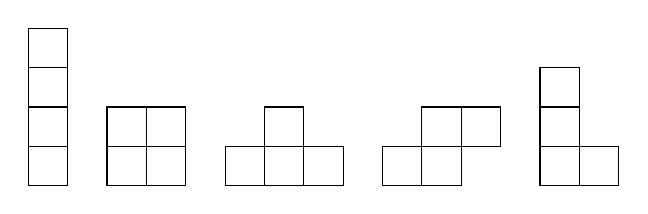
\begin{tikzpicture}[scale=0.5] % Verkleinere die Blöcke

% 4er Turm
\begin{scope}
\foreach \y in {0,1,2,3} {
  \draw (0,\y) rectangle (1,\y+1);
}
\end{scope}

% Abstand zwischen den Formen
\begin{scope}[shift={(2,0)}]
% Quadrat
\foreach \x in {0,1} {
  \foreach \y in {0,1} {
    \draw (\x,\y) rectangle (\x+1,\y+1);
  }
}
\end{scope}

% Abstand zwischen den Formen
\begin{scope}[shift={(5,0)}]
% Pyramide (T-Form)
\draw (0,0) rectangle (1,1);
\draw (1,0) rectangle (2,1);
\draw (2,0) rectangle (3,1);
\draw (1,1) rectangle (2,2);
\end{scope}

% Abstand zwischen den Formen
\begin{scope}[shift={(9,0)}]
\draw (0,0) rectangle (1,1);
\draw (1,0) rectangle (2,1);
\draw (1,1) rectangle (2,2);
\draw (2,1) rectangle (3,2);
\end{scope}

% Abstand zwischen den Formen
\begin{scope}[shift={(13,0)}]
% L-Form
\draw (0,0) rectangle (1,1);
\draw (0,1) rectangle (1,2);
\draw (0,2) rectangle (1,3);
\draw (1,0) rectangle (2,1);
\end{scope}

\end{tikzpicture} \]

For the questions below, we also allow these pieces to be "flipped over" and rotated. \\

\noindent (a) Is it possible to perfectly cover a $4 \times 5$ chessboard using each of these shapes exactly once? Prove that it is impossible, or show by example that it is possible.\\

\noindent (b) Is it possible to perfectly cover an $8 \times 5$ chessboard using each of these shapes exactly twice? Prove that it is impossible, or show by example that it is possible.\\

\subsubsection*{Solution}

(a) 
\begin{proof}
    Note that a $4 \times 5$ chessboard has $10$ squares of each color. To perfectly cover the chessboard, the pieces must cover exactly $10$ squares of each color. However, upon closer inspection of the shapes, we observe that they will always cover $11$ squares of one color and only $9$ squares of the other. This imbalance arises due to the small pyramid shape, which covers $3$ squares of one color and only $1$ square of the other. Hence, it is impossible to achieve a perfect cover.
    
\end{proof}

\noindent (b) 
\[
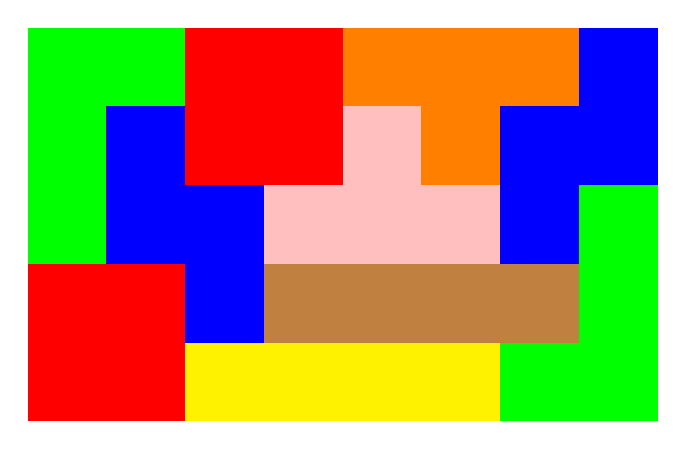
\begin{tikzpicture}

% Quadrate
\fill[red] (0,0) rectangle (2,2);   
\fill[red] (2,3) rectangle (4,5);   

%L
\fill[green] (0,2) rectangle (1,5);   
\fill[green] (1,4) rectangle (2,5);   

\fill[green] (6,0) rectangle (8,1);   
\fill[green] (7,1) rectangle (8,3);  

% Türme
\fill[yellow] (2,0) rectangle (6,1);   
\fill[brown] (3,1) rectangle (7,2);   

%S
\fill[blue] (1,2) rectangle (2,4);   
\fill[blue] (2,1) rectangle (3,3);   

\fill[blue] (6,2) rectangle (7,4);   
\fill[blue] (7,3) rectangle (8,5);   

%Pyramiden
\fill[pink] (3,2) rectangle (6,3);   
\fill[pink] (4,3) rectangle (5,4);  

\fill[orange] (4,4) rectangle (7,5);   
\fill[orange] (5,3) rectangle (6,4);  

\end{tikzpicture} \]

\newpage

\subsection{Exercise 1.5.}
\textbf{Task:} If I remove two squares of different colors from an $8 \times 8$ chessboard, must the result have a perfect cover?

\subsubsection*{Official Solution} 
Jay Cummings' \textcolor{blue}{\href{https://longformmath.com/proofs-hints-\%26-solutions}{solution}} to this exercise is wonderful! It is very long and I wanted to conclude my own proof, but you can look it up in "Chapter 1 Solutions to Selected Exercises" - Question 2.

\subsubsection*{Solution}

\begin{proof} Observe that the amount of squares between two opposite-colored squares on a chessboard is always an \textit{even} number, which can be perfectly covered using dominoes since each domino covers two squares.

To solve this problem, we connect the two removed squares and form a rectangle using dominoes, ensuring that the removed squares are located at opposite corners of this rectangle.

\begin{figure}[htbp] \centering \includegraphics[width=0.25\textwidth]{images/1.5.1.jpg}
\end{figure}

Since the horizontal or vertical distance between the two removed squares is always \textit{even}, we can fill the interior of the rectangle with dominoes by aligning them in rows or columns.

\begin{figure}[htbp] \centering \includegraphics[width=0.25\textwidth]{images/1.5.2.jpg} % \label{fig} 
\end{figure}

\newpage

Now, we have an $m \times n$ rectangle on the chessboard, where $m$ is an \textit{even} number and $n$ is an \textit{odd} number. Because one of the rectangle’s dimensions is even, the rectangle with the crossed-out squares can be viewed as a complete rectangle filled with dominoes, we can proceed to operate on it as such.

\begin{figure}[htbp] \centering \includegraphics[width=0.25\textwidth]{images/1.5.3.jpg} % \label{fig} 
\end{figure}

If we place dominoes in columns to fill the rectangle in the step before, the squares to the left and right of the rectangle can be filled with \textcolor{red}{vertical} dominoes, while the rest of the chessboard is covered with \textcolor{blue}{horizontal} dominoes.\\
If the dominoes in the rectangle are arranged in rows, we can simply rotate the chessboard by 90° and proceed as described for the column arrangement.\\

\begin{figure}[htbp] \centering \includegraphics[width=0.25\textwidth]{images/1.5.4.jpg} % \label{fig} 
\end{figure}

Therefore, when two squares of different colors are removed from an $8 \times 8$ chessboard, it is always possible to cover the remaining squares perfectly with dominoes. 
\end{proof}

\newpage

\subsection{Exercise 1.6.}
\textbf{Task:} If I remove four squares  $-$ two black, two white $-$ from an $8 \times 8$ chess board, must the result have a perfect cover?\\

\noindent $\longrightarrow$ If you believe a perfect cover must exist, justify why. \\

\noindent $\longrightarrow$ If you believe a perfect cover does not need to exist, give an example of four squares that you could remove for which the result does not have a perfect cover.

\subsubsection*{Solution}

The result does not need to have a perfect cover, as demonstrated by the example below. The bottom-left and bottom-right squares can no longer be covered by a domino because they are boxed in.

\begin{figure}[htbp] \centering \includegraphics[width=0.25\textwidth]{images/1.6.jpg} % \label{fig} 
\end{figure}

\noindent This chessboard can not be perfectly covered because no 2-square-long domino can cover a1 without also covering one of
the crossed-out squares a2 or b1.

\newpage

\subsection{Exercise 1.7.}
\textbf{Task:} In chess, a \textit{knight} is a piece that can move two squares vertically and one square horizontally, or two squares horizontally and one square vertically. A knight can legally move to any one of these squares, provided there is not another piece on that same square.\\

\noindent (a) Suppose there is a knight in every square of a $7 \times 7$ chessboard. Is it possible for every one of these knights to simultaneously make a legal move?\\

\noindent (b) Suppose there is a knight in every square of a $8 \times 8$ chessboard. Is it possible for every one of these knights to simultaneously make a legal move?

\subsubsection*{Solution}

(a) 

\begin{proof}
    Consider that a $7 \times 7$ chessboard has 49 squares, meaning there are 25 squares of one color and 24 squares of the opposite color. Thus, 25 knights are positioned on squares of one color, and 24 knights are on squares of the other color. \\
    Whenever a knight moves, it always lands on a square of the opposite color, as its move covers an odd number of squares. Therefore, all 25 knights that are on the more frequent color must move to the 24 squares of the less frequent color. \\
    However, by the pigeonhole principle, it is impossible to place 25 knights onto only 24 squares without at least one square being occupied by more than one knight, which is not allowed. \\
    Hence, it is impossible for all the knights on a $7 \times 7$ chessboard to make a legal move simultaneously.
\end{proof}

\noindent (b)

\begin{proof}
We start by demonstrating that this is possible on a $4 \times 2$ chessboard. In the diagram below, there are four pairs of knights, each pair occupying different colors. These knights can swap positions simultaneously. \\
\[
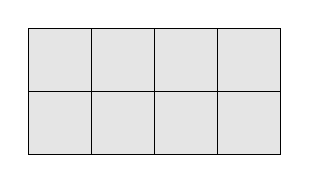
\begin{tikzpicture}[scale=0.8]

% Farben definieren
\definecolor{color1}{rgb}{1,0,0}   % Rot
\definecolor{color2}{rgb}{0,1,0}   % Grün
\definecolor{color3}{rgb}{0,0,1}   % Blau
\definecolor{color4}{rgb}{1,1,0}   % Gelb

% Schachbrett zeichnen
\foreach \x in {0,1,2,3} {
    \foreach \y in {0,1} {
        \fill[gray!20] (\x,\y) rectangle (\x+1,\y+1); 
        \draw (\x,\y) rectangle (\x+1,\y+1);
    }
}

% Springer und ihre Farben platzieren
\node at (0.5,1.5) {\textcolor{color1}{\Huge\knight}}; % Springer 1
\node at (1.5,1.5) {\textcolor{color2}{\Huge\knight}}; % Springer 2
\node at (2.5,1.5) {\textcolor{color3}{\Huge\knight}}; % Springer 3
\node at (3.5,1.5) {\textcolor{color4}{\Huge\knight}}; % Springer 4

\node at (0.5,0.5) {\textcolor{color3}{\Huge\knight}}; % Springer 3
\node at (1.5,0.5) {\textcolor{color4}{\Huge\knight}}; % Springer 4
\node at (2.5,0.5) {\textcolor{color1}{\Huge\knight}}; % Springer 1
\node at (3.5,0.5) {\textcolor{color2}{\Huge\knight}}; % Springer 2

\end{tikzpicture}
\] \\

\noindent Since the $4 \times 2$ chessboard fits exactly eight times within a standard $8 \times 8$ chessboard, we can apply this same swapping pattern across all the $4 \times 2$ sections of the larger board. Therefore, it is indeed possible for all knights on an $8 \times 8$ chessboard to make a legal move at the same time.

\end{proof}

\newpage

\subsection{Exercise 1.8.}
\textbf{Task:} Prove that if one chooses $n + 1$ numbers from $\{1,2,3,\dots,2n\}$, it is guaranteed that two of the numbers they chose are consecutive. Also, before your proof, write down an example of $4$ numbers from $\{1,2,3,4,5,6\}$ and locate two of them which are consecutive. Then, repeat for $5$ numbers from $\{1,2,3,\dots,8\}$ and $6$ numbers from $\{1,2,3,\dots,10\}$.

\subsubsection*{Solution}

\begin{proof}
    This problem can be addressed using the pigeonhole principle. To demonstrate the guarantee of selecting consecutive numbers, we can categorize the numbers from the set $\{1, 2, 3, \ldots, 2n\}$ into $n$ pairs, each representing a box of consecutive numbers:

    \[
    \fbox{1 and 2} \quad \fbox{3 and 4} \quad \fbox{5 and 6} \quad \dots \quad \fbox{2n-1 and 2n}
    \]

    By organizing the numbers in this manner, we create $n$ distinct pairs. When we choose $n + 1$ numbers from the set, the pigeonhole principle asserts that at least one pair (or box) must contain two numbers. Consequently, these two numbers must be consecutive.

    Therefore, it follows that if one chooses $n + 1$ numbers from $\{1, 2, 3, \ldots, 2n\}$, at least two of the chosen numbers will be consecutive.
\end{proof}

\subsection{Exercise 1.9.}
\textbf{Task:} Assume that $n$ is a positive integer. Prove that if one selects any $n + 1$ numbers from the set $\{1,2,3,\dots,2n\}$, then two of the selected numbers will sum to $2n+1$. Also, before your proof, write down an example of $4$ numbers from $\{1,2,3,4,5,6\}$ and locate two of them which sum to 7. Then, repeat for $5$ numbers from $\{1,2,3,\dots,8\}$ and $5$ numbers from $\{1,2,3,\dots,10\}$.

\subsubsection*{Solution}

\begin{proof}
    This problem can be addressed using the pigeonhole principle. To demonstrate the guarantee of selecting numbers, that sum up to $2n + 1$, we can categorize the numbers from the set $\{1, 2, 3, \ldots, 2n\}$ into $n$ pairs:

    \[
    \fbox{$1$ and $2n$} \quad \fbox{$2$ and $2n-1$} \quad \fbox{$3$ and $2n-2$} \quad \dots \quad \fbox{$n$ and $n+1$}
    \]

    By organizing the numbers in this manner, we create $n$ distinct pairs. When we choose $n + 1$ numbers from the set, the pigeonhole principle asserts that at least one pair (or box) must contain two numbers. Consequently, these two numbers must sum up to $2n+1$.

    Therefore, it follows that if one chooses $n + 1$ numbers from $\{1, 2, 3, \ldots, 2n\}$, at least two of the chosen numbers will must sum up to $2n+1$.
\end{proof}

\newpage

\subsection{Exercise 1.10.}
\textbf{Task:} Explain in your own words what the general pigeonhole principle says. 

\subsubsection*{Solution}

The pigeonhole principle states that if you place more objects than there are boxes, at least one box must contain more than one object. Specifically, if you place $n+1$ objects into $n$ boxes, then at least one box will contain at least two objects, because there are simply more objects than boxes. \\
The general form of the pigeonhole principle extends this idea: If you place $kn+1$ objects into $n$ boxes, then at least one box will contain at least $k+1$ objects This is because there are more objects than can be evenly distributed among the boxes, so at least one box must contain more than $k$ objects.

\subsection{Exercise 1.11.}
\textbf{Task:} Prove that there are at least two U.S. residents that have the same weight when rounded to the nearest \textit{millionth} of a pound. Hint: Do a Google search for how many U.S. residents weigh over 300 pounds.

\subsubsection*{Solution}

\begin{proof}
The United States had an official estimated resident population of \\335,893,238 on Jan 1, 2024, according to the U.S. Census Bureau. Given that 1.5\% of U.S. adults weigh over 300 pounds, approximately 5 million residents fall into this category. Thus, about 330 million U.S. residents weigh between 0 and 300 pounds. \\
Since there are only 300 million distinct weights when rounded to the nearest millionth of a pound in this range, by the pigeonhole principle, it is impossible to assign all 330 million residents distinct weights. Therefore, at least two residents must share the same weight when rounded to the nearest millionth of a pound. 
\end{proof}

\subsection{Exercise 1.12.}
\textbf{Task:} Determine whether or not the pigeonhole principle guarantees that two students at your school have the exact same 3-letter initials. (Include first, middle and last name in the initials. For instance, Natalie Laura Hobson = NLH).

\subsubsection*{Solution}

\begin{proof}
Currently, approximately 14,600 students are enrolled at my university. There are $26 \times 26 \times 26$ (17,576) possible 3-letter initials. Therefore, it is possible for each student to have a unique 3-letter initial.
\end{proof}

\newpage 

\subsection{Exercise 1.13.}
\textbf{Task:} Find your own real-world example of the pigeonhole principle.

\subsubsection*{Solution}

Consider a table tennis club with 30 players and a maximum of 20 possible racket brands. By the pigeonhole principle, since there are more players than brands, at least two players must be using the same brand of racket. Thus, it is impossible for all 30 players to use distinct racket brands, ensuring that at least two share a brand.

\subsection{Exercise 1.14.}
\textbf{Task:} Prove that if one chooses 31 numbers from the set $\{1,2,3,\dots,60\}$, that two of the numbers must be relatively prime.

\subsubsection*{Solution}

\begin{proof}
    Notice, that all consecutive numbers are always relatively prime. Using that fact, we can prove this proposition the same way we proved \textbf{Exercise 1.8}: \\
    To demonstrate the guarantee of selecting relatively prime numbers, we can categorize the numbers from the set $\{1, 2, 3, \ldots, 60\}$ into 31 pairs, each representing a box of relatively prime numbers:

    \[
    \fbox{1 and 2} \quad \fbox{3 and 4} \quad \fbox{5 and 6} \quad \dots \quad \fbox{59 and 60}
    \]

    By organizing the numbers in this manner, we create 31 distinct pairs. When we choose 31 numbers from the set, the pigeonhole principle asserts that at least one pair (or box) must contain two numbers. \\Consequently, these two numbers must be relatively prime.\\
    Therefore, it follows that if one chooses 31 numbers from $\{1, 2, 3, \ldots, 60\}$, at least two of the chosen numbers will be relatively prime.
\end{proof}

\newpage

\subsection{Exercise 1.15.} 
\textbf{Task:} Assume that $n$ is a positive integer. Prove that if one chooses any $n+1$ distinct odd integers from $\{1, 2, 3, \ldots, 3n\}$, then at least on of these numbers will divide another. Also, before your proof, check all possible selections of 4 odd numbers from $\{1, 2, 3, \ldots, 9\}$, and for each selection locate two of the numbers for which one divides another.

\subsubsection*{Solution}

\begin{proof}
 To prove that when selecting $n+1$ distinct odd numbers from the set $\{1, 2, 3, \ldots, 3n\}$, at least one number will divide another, we can group the numbers into $n$ pairs, where each box contains odd numbers that divide each other. \\
First, we remove the number 1 from the set, as it divides any other odd number. This is not an issue, because if 1 is selected along with any other odd number, then 1 will divide that number. Therefore, it suffices to focus on the remaining odd numbers. \\
We define the boxes as groups containing numbers of the form $k \cdot 3^m$, where $k$ is an odd positive integer greater than 1 and $m$ is a non-negative integer. \\
 

\underline{Case 1: $n$ is an \textbf{odd} positive integer}
    \[
    \fbox{3, 9, 27,\dots,$3*3^m$} \quad \fbox{5, 15, 45,\dots,$5*3^m$} \quad \dots \quad \fbox{$n$,$n*3^1$, $n*3^2$, \dots ,$n*3^m$}
    \]

\underline{Case 2: $n$ is an \textbf{even} positive integer}
    \[
    \fbox{3, 9, 27,\dots,$3*3^m$} \quad \fbox{5, 15, 45,\dots,$5*3^m$} \quad \dots \quad \fbox{$(n-1)$,$(n-1)*3^1$, \dots ,$(n-1)*3^m$}
    \] 

Notice that in both cases, there are $n$ boxes, and we are selecting $n+1$ numbers from the set $\{1, 2, 3, \ldots, 3n\}$. By the pigeonhole principle, at least one box must contain two numbers after selecting $n+1$ numbers. Since the numbers within a box are of the form $k \cdot 3^m$, one of them must divide the other. \\
Thus, if one chooses any $n+1$ distinct odd integers from $\{1, 2, 3, \ldots, 3n\}$, at least one of these numbers will divide another.
    
\end{proof}

\subsection{Exercise 1.16.} 
\textbf{Task:} Give an example of 100 numbers from $\{1, 2, 3, \ldots, 200\}$ such that none of your selected numbers divides any of the others. By doing so, this proves that Proposition 1.11 is optimal.

\subsubsection*{Solution}

$\{101, 102, 103, \ldots, 200\}$

\newpage

\subsection{Exercise 1.17.} 
\textbf{Task:} Prove that any set of seven integers contains a pair whose sum or difference is divisible by 10. Also, before your proof, write down three different sets of seven integers, and for each set locate a pair whose sum or difference is divisible by 10. Have your sets contain a diverse collection of integers - some bigger, some smaller, some positive, some negative.

\subsubsection*{Solution}

\begin{proof}
Observe that every integer ends in a digit between 0 and 9. A pair whose sum or difference is divisible by 10 is formed from two integers that either share the same last digit (Example: 56 and -36, where $56 + (-36) = 20$ and $20 \div 10 = 2$) or whose last digits add up to 10 (Example: 82 and 8, where $82 + 8 = 90$ and $90 \div 10 = 9$). With this in mind, we can categorize integers into the following six groups based on their last digit:

    \[
    \fbox{1 and 9} \quad \fbox{2 and 8} \quad \fbox{3 and 7} \quad \fbox{4 and 6} \quad \fbox{5} \quad \fbox{0}
    \]\\

Now, if we select 7 random integers and sort them by their last digit, placing them into the corresponding group, the pigeonhole principle guarantees that at least one group will contain two numbers. As demonstrated above, these two numbers will either have the same last digit or their last digits will sum to 10, ensuring that their sum or difference is divisible by 10.

\end{proof}

\newpage

\subsection{Exercise 1.18.} 
\textbf{Task:} Prove that if one chooses any 19 points from the interior of a $6 \times 4$ rectangle and no three form a straight line, then there must exist four of these points which form a quadrilateral area of at most 4.
\[
    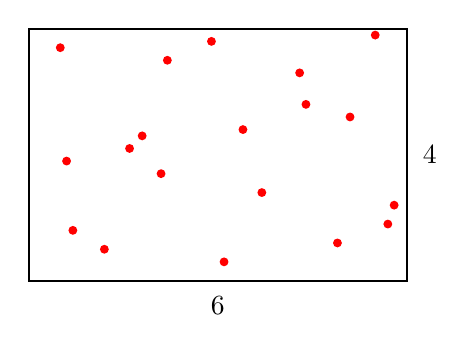
\begin{tikzpicture}[scale=0.8] 
    
    % Outline the rectangle
    \draw[thick] (0,0) rectangle (6,4);

    \draw (3,-0.1) node[below] {6}; % Bottom side
    \draw (6.1,2) node[right] {4};  % Right side
    
    % Plot 19 random points inside the rectangle
    \foreach \x/\y in {0.5/3.7, 1.8/2.3, 2.9/3.8, 3.7/1.4, 5.1/2.6, 1.2/0.5, 
                       4.3/3.3, 5.5/3.9, 0.7/0.8, 2.1/1.7, 3.4/2.4, 4.9/0.6,
                       0.6/1.9, 5.8/1.2, 3.1/0.3, 2.2/3.5, 1.6/2.1, 4.4/2.8, 5.7/0.9} {
        \fill[red] (\x,\y) circle (2pt);
    }
    \end{tikzpicture}
\]

\subsubsection*{Solution}

\begin{proof}
    Take the $6 \times 4$ rectangle and divide it into 6 $(2 \times 2)$ boxes as follows:

    \[
    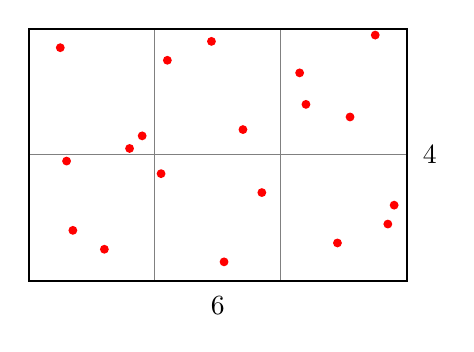
\begin{tikzpicture}[scale=0.8] 
    % Draw the grid
    \draw[step=2cm,gray,very thin] (0,0) grid (6,4);

    \draw (3,-0.1) node[below] {6}; % Bottom side
    \draw (6.1,2) node[right] {4};  % Right side
    
    % Outline the rectangle
    \draw[thick] (0,0) rectangle (6,4);
    
    % Plot 19 random points inside the rectangle
    \foreach \x/\y in {0.5/3.7, 1.8/2.3, 2.9/3.8, 3.7/1.4, 5.1/2.6, 1.2/0.5, 
                       4.3/3.3, 5.5/3.9, 0.7/0.8, 2.1/1.7, 3.4/2.4, 4.9/0.6,
                       0.6/1.9, 5.8/1.2, 3.1/0.3, 2.2/3.5, 1.6/2.1, 4.4/2.8, 5.7/0.9} {
        \fill[red] (\x,\y) circle (2pt);
    }
    \end{tikzpicture}
\]

As for the points on the lines between squares, consider them part of the square above and/or to the right. Doing this, each of the points in the $6 \times 4$ rectangle is assigned to one of the 6 boxes. By the pigeonhole principle, by placing 19 points into these 6 boxes, at least one box has at least 4 points in it.\\
The maximum quadrilateral area of four points in a $(2 \times 2)$ square is 4.
\[
    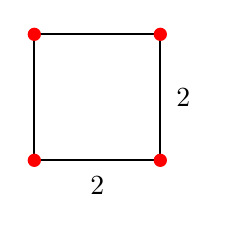
\begin{tikzpicture}[scale=0.8] 
    % Draw the square
    \draw[thick] (0,0) rectangle (2,2);
    
    % Label the sides
    \draw (1,-0.1) node[below] {2}; % Bottom side
    \draw (2.1,1) node[right] {2};  % Right side
    
    % Draw red points in each corner
    \fill[red] (0,0) circle (3pt);  % Bottom-left corner
    \fill[red] (2,0) circle (3pt);  % Bottom-right corner
    \fill[red] (0,2) circle (3pt);  % Top-left corner
    \fill[red] (2,2) circle (3pt);  % Top-right corner
    \end{tikzpicture}
\]

Hence, we are guaranteed that there is at least one $(2 \times 2)$ square with at least 4 points in it, there must exist four points which form a quadrilateral area of at most 4.

\end{proof}

\newpage

\subsection{Exercise 1.19.} 
\textbf{Task:} Assume that 9 points are chosen from the right triangle below and that no three of them form a straight line. Prove that there exist three of these points which form a triangle whose area is less than 1/2. 
\[
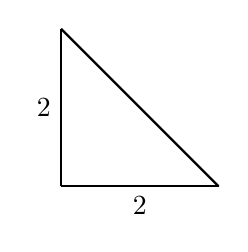
\begin{tikzpicture}
    % Draw the right triangle mirrored horizontally
    \draw[thick] (0,0) -- (0,2) node[midway, left] {2}; % Vertical side
    \draw[thick] (0,0) -- (2,0) node[midway, below] {2}; % Horizontal side
    \draw[thick] (0,2) -- (2,0) node[midway, above, sloped] {}; % Hypotenuse
\end{tikzpicture}
\]

\subsubsection*{Solution}

\begin{proof}
    Take the triangle and divide it into 4 triangles with a area of 1/2 each:

   \[
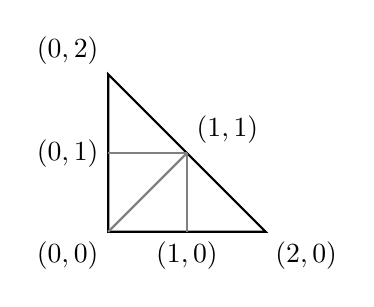
\begin{tikzpicture}
    % Draw the main triangle
    \draw[thick] (0,0) -- (0,2) -- (2,0) -- cycle;
    
    % Draw the internal lines to divide the triangle into four smaller triangles
    \draw[thick, gray] (0,1) -- (1,1); 
    \draw[thick, gray] (1,0) -- (1,1); 
    \draw[thick, gray] (0,0) -- (1,1); 
    
    % Label the points for clarity
    \node[below left] at (0,0) {$(0,0)$};
    \node[above left] at (0,2) {$(0,2)$};
    \node[below right] at (2,0) {$(2,0)$};
    \node[above right] at (1,1) {$(1,1)$};
    \node[below] at (1,0) {$(1,0)$};
    \node[left] at (0,1) {$(0,1)$};
\end{tikzpicture}
\]

   Now, consider the placement of 9 points within this large triangle. By the pigeonhole principle, if we place 9 points into these 4 smaller triangles, at least one of the smaller triangles must contain 3 or more points.

Since the area of each smaller triangle is $1/2$, and the maximum possible area of a triangle formed by three points within such a region is $1/2$, we are guaranteed that the area of any triangle formed by three points inside this small triangle will either be less than or equal to $1/2$.

Moreover, if the three points happen to lie on a straight line, which must be the case when in the small triangles the area of the 3 points is exactly 1/2 as shown below, their area is exactly 0.
Thus, we conclude that there must exist three points among the chosen 9 that form a triangle whose area is less than $1/2$.

    \[
    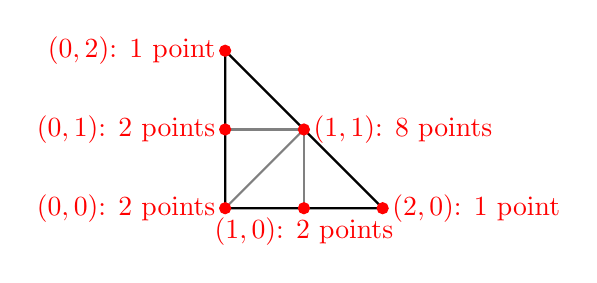
\begin{tikzpicture}
    % Draw the main triangle
    \draw[thick] (0,0) -- (0,2) -- (2,0) -- cycle;
    
    % Draw the internal lines to divide the triangle into four smaller triangles
    \draw[thick, gray] (0,1) -- (1,1); 
    \draw[thick, gray] (1,0) -- (1,1); 
    \draw[thick, gray] (0,0) -- (1,1); 
    
    % Add points along the edges forming a degenerate triangle
    \filldraw[red] (0,1) circle (2pt) node[left] {$(0,1)$: 2 points};
    \filldraw[red] (1,1) circle (2pt) node[right] {$(1,1)$: 8 points};
    \filldraw[red] (0,0) circle (2pt) node[left] {$(0,0)$: 2 points};
    \filldraw[red] (0,2) circle (2pt) node[left] {$(0,2)$: 1 point};
    \filldraw[red] (1,0) circle (2pt) node[below] {$(1,0)$: 2 points};
    \filldraw[red] (2,0) circle (2pt) node[right] {$(2,0)$: 1 point};
    
\end{tikzpicture}
\]

\end{proof}

\newpage

\subsection{Exercise 1.20.} 
\textbf{Task:} At a party, each person is \textit{acquainted} with a certain number of others at the party (and is a stranger to everyone else). For example, Jessica may be acquainted with six people at the party while Fara is acquainted with eight. Suppose that there are $\geq 2$ people at a party. Prove that at least two people at this party have the same number of acquaintances at the party. \\
You may also assume the following two things: \\
(1) Being acquaintances is symmetric (if John is acquainted with Heidi, then Heidi is also acquainted with John - no stalkers allowed at this party) and\\
(2) Every person is acquainted with at least one person at the party (no party crashers allowed).

\subsubsection*{Solution} 

\begin{proof} 
    Since every person is acquainted with at least one person at the party, the possible number of acquaintances are $1,2,3,\dots,(n-1)$, where $n$ is the total number of people at the party. Therefore, there are $n$ people and $n-1$ possible numbers of acquaintances.\\
    We can think of assigning each person to a "box" corresponding to the number of people they know, with the possible boxes being labeled $1,2,3,\dots,(n-1)$. This gives us:

    \[
    \fbox{1} \quad \fbox{2} \quad \fbox{3} \quad \dots \quad \fbox{$(n-2)$} \quad \fbox{$(n-1)$}
    \]\\

   Since we have $n$ people being placed into $n-1$ boxes, by the simple form of the pigeonhole principle two people must be placed into the same box, which means they have the same number of acquaintances.

\end{proof}

\newpage

\subsection{Exercise 1.21.} 
\textbf{Task:} \\(a) Determine the population of your hometown and how many non-balding people in your hometown, if any, are guaranteed to have the same number of hairs on their head, according to the pigeonhole principle. \\
(b) Determine, as best you can, the number of students who attended your high school while you were a senior. Then, determine how many of them, if any, are guaranteed to have the same birthday according to the pigeonhole principle.

\subsubsection*{Solution} 

(a) 
\begin{itemize}
    \item The average person has between 100,000 and 150,000 hairs on their head, and essentially everyone has under 200,000 hairs. So we will focus on people with at most 199,999 hairs.
    \item For the sake of this problem, we'll define "non-balding" to mean they have at least 50,000 strands of hair.
    \item On the 31.05.2024, there were 3,790,590 people living in Berlin. Assuming that 25\% of Berlin residents are balding, there are 947,647 non-balding people in Berlin.
\end{itemize}

\begin{proof}
    By the above facts, there are 2,842,943 non-balding people in Berlin. We can use the pigeonhole principle and imagine a box for every hair count between 50,000 and 199,999:

     \[
    \fbox{50,000} \quad \fbox{50,001} \quad \fbox{50,002} \quad \dots \quad \fbox{$199,998$} \quad \fbox{$199,999$}
    \]\\

    Therefore there are 150,000 ($n$) boxes in which we put all names of the 2,842,943 ($kn+1$) people living in Berlin in the box with their hair count on it. By the pigeonhole principle we are guaranteed that there is at least one box with at least 18 $(k+1)$ names on it, meaning they have the same number of hairs on their head.

\end{proof}

\noindent (b)
\begin{proof} 
Assume that there were 900 students at my high school during my senior year and there are 366 possible birthdays. According to the pigeonhole principle, it is guaranteed that at least two students must share the same birthday, since the number of students exceeds the number of possible birthdays. 
\end{proof}

\newpage

\subsection{Exercise 1.22.} 
\textbf{Task:} The following conjectures are all false. Prove that they are false by finding a counterexample to each. \\

\noindent (a) \underline{Conjecture 1:} If $x$ and $y$ are real numbers, then $\lvert x + y \rvert = \lvert x \rvert + \lvert y \rvert$

\noindent (b) \underline{Conjecture 2:} If $x$ is a real number, then $x^2 < x^4$

\noindent (c) \underline{Conjecture 3:} Suppose $x$ and $y$ are real numbers. If $\lvert x + y \rvert = \lvert x - y \rvert$, then $y = 0$. 
 
\subsubsection*{Solution}

(a) $x := 1$ and $y:= -1$\\
(b) $x:= 0.1$\\
(c) $x := 0$ and $y:= 1$

\subsection{Exercise 1.23.} 
\textbf{Task:} Suppose you deal a pile of cards, face down, from a shuffled deck of cards (this is a standard 52-card deck, where each card is one of 4 suits and of 13 ranks). How many must you deal out until you are guaranteed \dots\\

\noindent (a) five of the same suit?\\
(b) two of the same rank?\\
(c) three of the same rank?\\
(d) four of the same rank?\\
(e) two of one rank and three of another?

\subsubsection*{Solution}

By applying the pigeonhole principle, we get:

\noindent(a) 17\\
(b) 14\\
(c) 27\\
(d) 40\\
(e) $4 + 13 = 17$\\

\newpage

\subsection{Exercise 1.24.} 
\textbf{Task:} Determine the U.S. population at the time you are reading this.\\
(a) Does the pigeonhole principle guarantee that 1 million U.S. residents all have the same birthday?\\
(b) If the principle does not guarantee this, how many people are needed until that milestone is reached? If the USA grows 2 million people per year, in what year will this occur?

\subsubsection*{Solution}

The United States had an official estimated resident population of 335,893,238 on Jan 1, 2024, according to the U.S. Census Bureau. \\

\noindent (a) To be guaranteed that 1 million U.S. residents all have the same birthday, there would have to be at least 366,000,001 U.S. residents. Since 335,893,238 $<$ 366,000,001, it's not guaranteed that 1 million U.S. residents all have the same birthday.\\

\noindent (b) To guarantee that 1 million U.S. residents all share the same birthday, we need a total population of 366,000,001. Assuming a growth rate of 2 million residents per year, we can determine the number of years required to reach this population by solving the following equation: 
\[
366,000,001 = 335,893,238 + 2x
\]
Solving for \(x\), we find \(x = 15,053,381.5\). Thus, it would take approximately 15,053,382 years to ensure that 1 million U.S. residents share the same birthday.

\newpage

\subsection{Exercise 1.25.} 
\textbf{Task:} Imagine a friend gives you a deck of cards (a standard 52-card deck) and lets you shuffle it a few times. They then ask you to slowly deal out the cards, one at a time, into a new pile on the table. The entire time the cards are face-down, so they have no idea which cards you are dealing.

At a certain point this procedure, they ask you to stop, and declare with confidence that the two stacks - the one still in your hand, and the one on the table - are in perfect balance. They say that the number of red cards in the stack in your hand is equal to the number of black cards in the stack on the table. They let you count, and sure enough, they were correct!

There were no gimmicks in this procedure - no trick cards or hidden cameras outside help. How did your friend do it?

\subsubsection*{Solution}

My friend always stops me after I’ve dealt the 26th card. To understand why this trick works, let’s define the number of black cards on the table as \(b\) and the number of red cards on the table as \(a\). The total number of cards dealt on the table is \(c = a + b\). Notice that the number of black cards is \(b = c - a\).\\
The number of red cards remaining in my hand is always \(26 - a\), because we start with 26 red cards and subtract the number of red cards dealt so far. Since the goal is for the number of black cards on the table to be equal to the number of red cards in my hand, we can set up the following equation:

\[
26 - a = c - a
\]

Simplifying this gives:

\[
26 = c
\]

Thus, when 26 cards have been dealt, the number of red cards remaining in my hand will always equal the number of black cards on the table. That’s why my friend can confidently stop me after the 26th card!

\newpage

\subsection{Exercise 1.26.} 
\textbf{Task:} An alien creature has three legs, and on each of his three alien feet he wears an alien sock. Suppose, he just washed $n$ triplets of alien sock ($3n$ individuals), and each triplet is a different color. If this alien pulls his alien socks out of his alien dryer one-at-a-time, how many must he pull to be guaranteed to have a matching triplet?

\subsubsection*{Solution}

To guarantee that the alien has pulled out a complete triplet of matching socks, the alien must pull out at least \(2n+1\) individual socks. This result follows from the pigeonhole principle. The principle states that if we place \(kn+1\) objects (in this case, \(2n+1\) individual socks) into \(n\) boxes (where each box represents a different color), at least one box will contain at least \(k+1\) objects (in this case, at least 3 socks of the same color). Therefore, after pulling out \(2n+1\) socks, the alien is guaranteed to have a matching triplet.

\newpage

\subsection{Exercise 1.27.} 
\textbf{Task:} A \textit{magic square} is an $n \times n$ matrix where the sum of the entries in each row, column or diagonal equal the same value. For example,

\[
\begin{bmatrix}
    8 & 1 & 6 \\
    3 & 5 & 7 \\
    4 & 9 & 2
\end{bmatrix}
\]

is a $3 \times 3$ matrix whose three rows, three columns, and two diagonals each sum up to 15. Thus, this is a magic square.

An \textit{antimagic square} is an $n \times n$ matrix where each row, column and diagonal sums to a distinct value. For example, 

\[
\begin{bmatrix}
    9 & 4 & 5 \\
    10 & 3 & -2 \\
    6 & 9 & 7
\end{bmatrix}
\]

is a $3 \times 3$ matrix, whose rows sum to 18, 11 and 22, columns sum to 25,16 and 10 and diagonals sum to 19 and 14. Notice that all eight of these numbers is different than the rest, showing that this is an antimagic square.

Prove that, for every $n$, there does not exist an $n \times n$ antimagic square where each entry is $-1,0$ or 1.

\subsubsection*{Solution}

\begin{proof}
    Observe that every $n \times n$ matrix has $n$ rows, $n$ columns, and 2 diagonals. Therefore, an antimagic square of size $n \times n$ has $2n+2$ sums (one for each row, column, and diagonal). To show that it is impossible for all these sums to be distinct when the matrix entries are $-1, 0$, or $1$, we can create a box for each possible result of adding $n$ entries, where each entry is $-1, 0$, or $1$. These possible results are:

    \[
    \fbox{-n} \quad \fbox{-n+1} \quad \fbox{-n+2} \quad \dots \quad \fbox{n-1} \quad \fbox{n}
    \]\\

    Notice that there are $2n+1$ such boxes, meaning there are $2n+1$ possible sums for all rows, columns, and diagonals. Since we need to place $2n+2$ sums into one of these $2n+1$ boxes, by the pigeonhole principle, at least one box must contain more than one sum. This implies that at least two rows, columns, or diagonals must have the same sum.\\
    Therefore, there cannot exist an $n \times n$ antimagic square where each entry is $-1, 0$, or $1$.
\end{proof}

\newpage

\subsection{Exercise 1.28.} 
\textbf{Task:} Read the \textit{Introduction to Ramsey Theory} following this chapter. Then, let $r(n,m)$ be the smallest value $N$ for which every red/blue coloring of $K_N$ contains either a red $K_n$ or a blue $K_m$. Prove that $r(n,2)=n$.

\subsubsection*{Solution}

\begin{proof}
To prove this proposition, we need to show that \( r(n,2) = n \), meaning that for any red/blue coloring of the edges of a complete graph \( K_N \), there is always either a red complete subgraph \( K_n \) or a blue edge \(K_2\), and the smallest such \(N\) is \( n \).

First, observe that any complete graph \( K_N \) for \( N \geq 2 \) must have at least one edge, which corresponds to a \( K_2 \) (a connection between two vertices). In a red/blue coloring of the edges, this \( K_2 \) will either be red or blue.

Next, let's consider the case when \( N = 1 \). Notice that a \( K_2 \) cannot exist within a \( K_1 \), as the latter has only one vertex. Therefore, \( n \) cannot be 1 and must be at least 2. 

Finally, to show that \( r(n,2) = n \), consider a complete graph \( K_N \) for \( N \geq 2 \). As demonstrated earlier, the smallest possible subgraph in this \( K_N \) is a \( K_2 \). Therefore, any other subgraph \( K_n \) within this complete graph must also be at least a \( K_2 \) or larger.

This completes the proof that \( r(n,2) = n \).
\end{proof}

\newpage

\section{Chapter 2: Direct Proofs}

\subsection{Exercise 2.1.}
\textbf{Task:} List 5 skills that are important for someone to be successful in a college math class. Which skills seem most important for an upper-division math class? Which skills do you want to work to improve?

\subsubsection*{Solution}

\underline{5 skills that are important for success in a college math class:}\\
- understanding the solution process for various types of problems\\
- minimizing computational mistakes\\
- staying organized and managing time effectively\\
- thoroughly reviewing and understanding prerequisite concepts\\
- consistently practicing and solving similar types of problems\\

\noindent \underline{5 skills that are important for success in an upper-division math class:}\\
- writing clear and rigorous proofs\\
- effectively communicating mathematical ideas\\
- analyzing abstract concepts and definitions in detail\\
- integrating different areas of mathematics\\
- applying creativity in proof-writing and problem-solving\\

\noindent I want to work on improving my communication skills, especially in written form. I would also love to approach some problems in this book with creative solutions.


\newpage

\subsection{Exercise 2.2.}
\textbf{Task:} The following are the squares of four numbers, each ending in a 5.

\begin{align*}
    15^2 &= 225\\
    25^2 &= 625\\
    35^2 &= 1225\\
    45^2 &= 2025\\
\end{align*}

\noindent Looking at these four squares, do you see anything interesting about their answers? Once you have noticed a pattern, answer the following:\\

\noindent (a) Write down a conjecture that explains what the answer is for the square of any integer ending in a 5.\\
(b) Give four more examples illustrating your conjecture.\\
(c) Prove your conjecture.\\

\subsubsection*{Solution}

(a)

\begin{conjecture}{}
   If a number is ending in a 5, the square of this number will always end in a 25.
\end{conjecture}

\noindent (b)

\begin{align*}
    85^2 &= 7225\\
    125^2 &= 15625\\
    232813785^2 &= 54202258486026225\\
    3184712894812745^2 &= 10142396222386574198728614435025\\
\end{align*}

\noindent (c)

\begin{proof}
Let’s consider any number that ends in 5. Such a number can always be expressed in the form \( 10n + 5 \), where \( n \) is an integer. Now, let’s square this number:
\[
(10n + 5)^2 = 100n^2 + 100n + 25 = 100(n^2 + n) + 25.
\]
Notice that \( 100(n^2 + n) \) is always a multiple of 100, which means it ends in two zeros. Adding 25 to this result gives a number that ends in 25, since \( 0 + 25 = 25 \).

Thus, the square of any number ending in 5 will always end in 25, as required.
\end{proof}


\subsection{Exercise 2.3.}
\textbf{Task:} For each of the following, give three examples of this property. Then, prove that it is true.

\noindent (a) The sum of an even integer and an odd integer is odd;\\
(b) The product of two even integers is even;\\
(c) The product of two odd integers is odd;\\
(d) The product of an even integer and an odd integer is even;\\
(e) An even integer squared is an even integer

\subsubsection*{Solution}

(a)
\begin{proof}
    Assume that $n$ is an even integer and $m$ is an odd integer. By Definition 2.2, this means that $n=2a$ and $m=2b+1$, for some integers $a$ and $b$. Then,

\[n+m=(2a)+(2b+1)=2a+2b+1=2(a+b)+1.\]

    And since, by Fact 2.1, $(a+b)$ is an integer too, we have shown that $n+m=2k+1$, where $k=a+b$ is an integer. Therefore, by Definition 2.2, this means that $n+m$ is odd.
\end{proof}

\noindent(b)

\begin{proof}
    Assume that $n$  and $m$ are even integers. By Definition 2.2, this means that $n=2a$ and $m=2b$, for some integers $a$ and $b$.
    Then,

    \[n \cdot m=(2a)\cdot(2b)=4ab=2(2ab)\]

    And since, by Fact 2.1 $2ab$ is an integer too, we have shown that $n\cdot m=2k$, where $k=2ab$ is an integer. Therefore, by Definition 2.2, this means that $n \cdot m$ is even.
\end{proof}
    
\noindent(c)

\begin{proof}
    Assume that $n$  and $m$ are odd integers. By Definition 2.2, this means that $n=2a+1$ and $m=2b+1$, for some integers $a$ and $b$.
    Then,

   \[n \cdot m=(2a+1)\cdot(2b+1)=4ab+2a+2b+1=2(2ab+a+b)+1\]

   And since, by Fact 2.1 $2ab+a+b$ is an integer too, we have shown that $n\cdot m=2k+1$, where $k=2ab+a+b$ is an integer. Hence, by Definition 2.2, this means that $n \cdot m$ is odd.
\end{proof}

\newpage

\noindent(d)

\begin{proof}
    Assume that $n$ is an even integer and $m$ is an odd integer. By Definition 2.2, this means that $n=2a$ and $m=2b+1$, for some integers $a$ and $b$. Then,

    \[n\cdot m=(2a)\cdot(2b+1)=4ab+2a=2(2ab+a).\]

    And since, by Fact 2.1 $2ab+a$ is an integer too, we have shown that $n\cdot m=2k$, where $k=2ab+a$ is an integer. Therefore, by Definition 2.2, this means that $n \cdot m$ is even.
\end{proof}

\noindent(e)

\begin{proof}
    Assume that $n$ is an even integer. By Definition 2.2, this means that $n=2a$, for some integer $a$. Then,

    \[n^2=(2a)^2=4a^2=2(2a^2)\]

    And since, by Fact 2.1, $2a^2=2 \cdot a \cdot a$ is an integer too, we have shown that $n^2=2k$, where $k=2a^2$ is an integer. Therefore, by Definition 2.2, this means that $n^2$ is even.
\end{proof}

\subsection{Exercise 2.4.} 
\textbf{Task:} For each of the following give three examples of this property. Then, prove that it is true.

\noindent (a) If $n$ is an even integer then, $-n$ is an even integer.\\
(b) If $n$ is an odd integer then, $-n$ is an odd integer. \\
(c) If $n$ is an even integer, then $(-1)^n=1$. You may use standard properties of exponents.

\subsubsection*{Solution}

(a) 

\begin{proof}
    Assume that $n$ is an even integer. By Definition 2.2, this means that $n=2a$, for some integer $a$. Then,

    \[(-n)=-(2a)=2(-a)\]

    And since $-a$ is an integer too, we have shown that $(-n)=2k$, where $k=-a$ is an integer. Therefore, by Definition 2.2, this means that $(-n)$ is even.
    
\end{proof}

\newpage

\noindent (b) 

\begin{proof}
    Assume that $n$ is an odd integer. By Definition 2.2, this means that $n=2a+1$, for some integer $a$. Then,

    \[(-n)=-(2a+1)=2(-a-1)+1\]

    And since, by Fact 2.1, $-a-1$ is an integer too, we have shown that $(-n)=2k+1$, where $k=(-a-1)$ is an integer. Therefore, by Definition 2.2, this means that $(-n)$ is odd.
\end{proof}

\noindent (c) 

\begin{proof}
    Assume that $n$ is an even integer. By Definition 2.2, this means that $n=2a$, for some integer $a$. Then,

   \[(-1)^n = (-1)^{(2a)} = ((-1)^{2})^{a} = 1^{a} = 1 \cdot 1 \cdot 1 \dots 1 = 1.\]

     Therefore, if $n$ is an even integer, then $(-1)^a = 1$, as required.
\end{proof}

\subsection{Exercise 2.5.} 
\textbf{Task:} Prove the following. For each, $n$ is an integer.\\
(a) If $n$ is odd, then $n^2+4n+9$ is even.\\
(b) If $n$ is odd, then $n^3$ is odd.\\
(c) If $n$ is even, them $n+1$ is odd.\\

\subsubsection*{Solution}

(a)

\begin{proof}
    Assume that $n$ is an odd integer. By Definition 2.2, this means that $n=2a+1$, for some integer $a$. Then,

    \[n^2+4n+9=(2a+1)^2+4(2a+1)+9=4a^2+4a+1+8a+8+9=4a^2+12a+18=2(2a^2+6a+9)\].

    And since, by Fact 2.1, $(2a^2+6a+9)$ is an integer too, we have shown that $(n^2+4n+9)=2k$, where $k=(2a^2+6a+9)$ is an integer. Therefore, by Definition 2.2, this means that $(n^2+4n+9)$ is even.
\end{proof}

\newpage

\noindent (b)

\begin{proof}
    Assume that $n$ is an odd integer. By Definition 2.2, this means that $n=2a+1$, for some integer $a$. Then,

    \[n^3=(2a+1)^3=8a^3+12a^2+6a+1=2(4a^3+6a^2+3a)+1\].

    And since, by Fact 2.1, $(4a^3+6a^2+3a)$ is an integer too, we have shown that $n^3=2k+1$, where $k=(4a^3+6a^2+3a)$ is an integer. Therefore, by Definition 2.2, this means that $n^3$ is odd.
\end{proof}

\noindent (c)

\begin{proof}
     Assume that $n$ is an even integer. By Definition 2.2, this means that $n=2a$, for some integer $a$. Then,

    \[n+1=(2a)+1=2(a)+1\].

    And since $a$ is an integer too, we have shown that $n+1=2k+1$, where $k=a$ is an integer. Therefore, by Definition 2.2, this means that $n+1$ is odd. 
\end{proof}

\subsection{Exercise 2.6.} 
\textbf{Task:} Prove the following. For each, $m$ and $n$ are integers.\\
(a) If $m$ and $n$ are odd, then $5m-3n$ is even.\\
(b) If $m$ and $n$ are even, then $3mn$ is divisible by 4.

\subsubsection*{Solution}

(a)

\begin{proof}
    Assume that $n$ and $m$ are odd integers. By Definition 2.2, this means that $n=2a+1$ and $m=2b+1$, for some integers $a$ and $b$. Then,

    \[5m-3n=5(2b+1)-3(2a+1)=10b+5-6a-3=10b-6a+2=2(5b-3a+1)\].

    And since, by Fact 2.1, $(5b-3a+1)$ is an integer too, we have shown that $5m-3n=2k$, where $k=(5b-3a+1)$ is an integer. Therefore, by Definition 2.2, this means that $5m-3n$ is even.
\end{proof}

\newpage

\noindent (b)

\begin{proof}
     Assume that $n$ and $m$ are even integers. By Definition 2.2, this means that $n=2a$ and $m=2b$, for some integers $a$ and $b$. Then,

     \[3mn=3(2b)(2a)=3(4ab)=4(3ab)\].

     And since, by Fact 2.1, $(3ab)$ is an integer too, we have shown that $3mn=4k$, where $k=(3ab)$ is an integer. Therefore, by Definition 2.8, this means that 4 divides $3mn$.
\end{proof}

\subsection{Exercise 2.7.}
\textbf{Task:} Provide a second proof of Proposition 2.7 in which you first prove that $n(n+1)$ is even, and then you apply Proposition 2.4.

\subsubsection*{Solution}

\begin{proof}
    Assume that $n$ is an integer. To prove that $n^2 + n + 6$ always results in an even number, we will first show that $n(n+1)$ is even. Since $n$ can be either odd or even, we consider both cases:\\
    
    \noindent \underline{\textbf{Case 1:} $n$ is an \textbf{even} number.}
    
    \noindent If $n$ is even, by Definition 2.8, we can write $n = 2a$ for some integer $a$. Then,
    
    \[
    n(n+1) = (2a)((2a)+1) = 4a^2 + 2a = 2(2a^2 + a).
    \]
    
    Since $2a^2 + a$ is an integer, we conclude that $n(n+1) = 2k$, where $k = 2a^2 + a$ is an integer. Therefore, by Definition 2.2, $n(n+1)$ is even.\\
    
    \noindent \underline{\textbf{Case 2:} $n$ is an \textbf{odd} number.}
    
    \noindent If $n$ is odd, by Definition 2.8, we can write $n = 2a + 1$ for some integer $a$. Then,
    \[
    n(n+1) = (2a+1)((2a+1)+1) = 4a^2 + 6a + 2 = 2(2a^2 + 3a + 1).
    \]
    
    Since $2a^2 + 3a + 1$ is an integer, we conclude that $n(n+1) = 2k$, where $k = 2a^2 + 3a + 1$ is an integer. Therefore, by Definition 2.2, $n(n+1)$ is even.
    
    This shows that $n(n+1)$ is even for all integers $n$, since every integer is either even or odd.
    
    Now, observe that $n(n+1) = n^2 + n$, which is always even as shown above. By Proposition 2.4, the sum of two even integers is always even. Since both $n^2 + n$ and 6 are even, their sum $n^2 + n + 6$ is also even.
\end{proof}

\newpage

\subsection{Exercise 2.8.}
\textbf{Task:} Give an example of each of the following properties. Then, prove that it is true.\\
(a) If $n$ is an integer, then $n^2+n$ is even.\\
(b) If $n$ is an integer, then $3n^2+5n+1$ is odd.\\
(c) If $n$ is an integer, then $n^2+3n-6$ is even.\\
(d) If $m$ and $n$ are integers of the same parity, them $7m-3n$ is even.

\subsubsection*{Solution}

(a) Since $n(n+1) = n^2 + n$, this task is shown first in Exercise 2.7.\\
(b) 

\begin{proof}
    Assume that $n$ is an integer. Since $n$ can be either odd or even, we consider both cases:\\

    \noindent \underline{\textbf{Case 1:} $n$ is an \textbf{even} number.}
    
    \noindent If $n$ is even, by Definition 2.8, we can write $n = 2a$ for some integer $a$. Then,

    \[3n^2+5n+1=3(2a)^2+5(2a)+1=12a^2+10+1=2(6a^2+5)+1\].

    And since, by Definition 2.2, $(6a^2+5)$ is an integer too, we have shown that $3n^2+5n+1=2k+1$, where $k=(6a^2+5)$ is an integer. Therefore, by Definition 2.2, this means that $3n^2+5n+1$ is odd. \\

    \noindent \underline{\textbf{Case 2:} $n$ is an \textbf{odd} number.}
    
    \noindent If $n$ is even, by Definition 2.8, we can write $n = 2a+1$ for some integer $a$. Then,

    \[3n^2+5n+1=3(2a+1)^2+5(2a+1)+1=3(4a^2+4a+1)+10a+5+1=12a^2+14a+7=2(6a^2+7a+3)+1\].

    And since, by Fact 2.1, $(6a^2+7a+3)+$ is an integer too, we have shown that $3n^2+5n+1=2k+1$, where $k=(6a^2+7a+3)+$ is an integer. Therefore, by Definition 2.2, this means that $3n^2+5n+1$ is odd. \\

    This shows that $3n^2+5n+1$ is odd for all integers $n$.
\end{proof}

\newpage

\noindent(c)

\begin{proof}
    Assume that $n$ is an integer. Since $n$ can be either odd or even, we consider both cases:\\

    \noindent \underline{\textbf{Case 1:} $n$ is an \textbf{even} number.}
    
    \noindent If $n$ is even, by Definition 2.8, we can write $n = 2a$ for some integer $a$. Then,

    \[n^2+3n-6=(2a)^2+3(2a)-6=2(2a^2+3a-3)\].

    And since, by Fact 2.1, $(2a^2+3a-3)$ is an integer too, we have shown that $n^2+3n-6=2k$, where $k=(2a^2+3a-3)$ is an integer. Therefore, by Definition 2.2, this means that $n^2+3n-6$ is even.\\

    \noindent \underline{\textbf{Case 2:} $n$ is an \textbf{odd} number.}
    
    \noindent If $n$ is even, by Definition 2.8, we can write $n = 2a+1$ for some integer $a$. Then,

    \[n^2+3n-6=(2a+1)^2+3(2a+1)-6=4a^2+4a+1+6a+3-6=2(2a^2+5a-1)\].

    And since, by Fact 2.1, $(2a^2+5a-1)$ is an integer too, we have shown that $n^2+3n-6=2k$, where $k=(2a^2+5a-1)$ is an integer. Therefore, by Definition 2.2, this means that $n^2+3n-6$ is even.\\

    This shows that $n^2+3n-6$ is even for all integers $n$.
\end{proof}

\noindent(d)

\begin{proof}
    Assume that $m$ and $n$ are integers of the same parity. Since $m$ and $n$ can be either both odd or even, we consider both cases:\\

    \noindent \underline{\textbf{Case 1:} $m$ and $n$ are \textbf{even} integers.}

    \noindent If $m$ and $n$ are even, by Definition 2.8, we can write $m = 2a$ and $n=2b$ for some integers $a$ and $b$. Then,

    \[7m-3n=7(2a)-3(2b)=2(7a-3b)\].

    And since, by Fact 2.1, $(7a-3b)$ is an integer too, we have shown that $7m-3n=2k$, where $k=(7a-3b)$ is an integer. Therefore, by Definition 2.2, this means that $7m-3n$ is even.\\

    \noindent \underline{\textbf{Case 2:} $m$ and $n$ are \textbf{odd} integers.}

    \noindent If $m$ and $n$ are even, by Definition 2.8, we can write $m = 2a+1$ and $n=2b+1$ for some integers $a$ and $b$. Then,

    \[7m-3n=7(2a+1)-3(2b+1)=2(7a-3b+2)\].

    And since, by Fact 2.1, $(7a-3b+2)$ is an integer too, we have shown that $7m-3n=2k$, where $k=(7a-3b+2)$ is an integer. Therefore, by Definition 2.2, this means that $7m-3n$ is even.\\

    This shows that $7m-3n$ is even for all integers $n$.
\end{proof}

\subsection{Exercise 2.9.}
\textbf{Task:} Determine conditions on integers $m$ and $n$ for which $mn$ is even. Write down your conditions as a conjecture, and then prove that your conjecture is correct.

\subsubsection*{Solution}

\begin{proof}
    To prove this conjecture, we need to consider three cases:
    
    \noindent \underline{\textbf{Case 1:} \textit{\(m\) is even and \(n\) is odd.}}
    
    If \(m\) is even and \(n\) is odd, then by Definition 2.8, we can express \(m = 2a\) and \(n = 2b + 1\) for some integers \(a\) and \(b\). Thus,
    
    \[
    mn = (2a)(2b + 1) = 4ab + 2a = 2(2ab + a).
    \]
    
    Since \(2ab + a\) is an integer by Fact 2.1, we have shown that \(mn = 2k\), where \(k = 2ab + a\) is an integer. Therefore, by Definition 2.2, \(mn\) is even.
    
    \noindent \underline{\textbf{Case 2:} \textit{\(m\) is odd and \(n\) is even.}}
    
    If \(m\) is odd and \(n\) is even, then by Definition 2.8, we can write \(m = 2a + 1\) and \(n = 2b\) for some integers \(a\) and \(b\). Therefore,
    
    \[
    mn = (2a + 1)(2b) = 4ab + 2b = 2(2ab + b).
    \]
    
    Since \(2ab + b\) is an integer by Fact 2.1, we have shown that \(mn = 2k\), where \(k = 2ab + b\) is an integer. Therefore, by Definition 2.2, \(mn\) is even.
    
    \noindent \underline{\textbf{Case 3:} \textit{Both \(m\) and \(n\) are even.}}
    
    If both \(m\) and \(n\) are even, then by Definition 2.8, we can express \(m = 2a\) and \(n = 2b\) for some integers \(a\) and \(b\). Thus,
    
    \[
    mn = (2a)(2b) = 4ab = 2(2ab).
    \]
    
    Since \(2ab\) is an integer by Fact 2.1, we have shown that \(mn = 2k\), where \(k = 2ab\) is an integer. Therefore, by Definition 2.2, \(mn\) is even.
    
    Thus, we have shown that \(mn\) is even whenever at least one of \(m\) or \(n\) is an even integer.
\end{proof}

\newpage

\subsection{Exercise 2.10.}
\textbf{Task:} Prove the following. For each, $m$, $n$ and $t$ are integers.\\
(a) If $m \mid n$, then $m^2 \mid n^2$.\\
(b) If $m \mid n$, then $m \mid (7n^3+13n^2-n)$.\\
(c) If $m \mid n$ and $m \mid t$, then $m \mid (n+t)$.\\
(d) If $3 \mid 2n$, then $3 \mid n$.\\
(e) If $9 \mid 6n$, then $3 \mid n$.\\
(f) If $m^3 \mid n$ and $n^4 \mid t$, then $m^{12} \mid t$.\\

\subsubsection*{Solution}

(a) 

\begin{proof}
    Assume that  $m \mid n$. By Definition 2.8, this means that $n=mk$ for some integer $k$.
    Thus,

    \[n^2=(mk)^2=m^2(k^2)\]

    We have shown that $n^2=m^2(k^2)$, and $(k^2=k\cdot k)$ is an integer. So it is indeed true that $n^2=m^2p$ for the integer $p=(k^2)$, which by the definition of divisibility (Definition 2.8) means $m^2 \mid n^2$.
\end{proof}

\noindent (b)

\begin{proof}
    Assume that  $m \mid n$. By Definition 2.8, this means that $n=mk$ for some integer $k$.
    Thus,

    \[7n^3+13n^2-n=7(mk)^3+13(mk)^2-(mk)=m(7m^2k^3+13mk^2-k)\]

    We have shown that $7n^3+13n^2-n=m(7m^2k^3+13mk^2-k)$, and ${(7m^2k^3+13mk^2-k)}$ is an integer. So it is indeed true that $7n^3+13n^2-n=mp$ for the integer $p=(7m^2k^3+13mk^2-k)$, which by the definition of divisibility (Definition 2.8) means $m \mid 7n^3+13n^2-n$.
\end{proof}

\noindent (c)

\begin{proof}
    Assume that  $m \mid n$ and $m \mid t$. By Definition 2.8, this means that $n=mk$ and $t=ms$ for some integers $k$ and $s$.
    Thus,

    \[n+t=mk+ms=m(ks)\]

    We have shown that $n+1=m(ks)$, and since $k$ and $s$ are integers, so is $ks$ by Fact 2.1. So it is indeed true that $n+1=mp$ for the integer $p=(ks)$, which by the definition of divisibility (Definition 2.8) means $m \mid n+1$.
\end{proof}

\newpage

\noindent (d) 

\begin{proof}
    Assume that $ 3 \mid 2n $ and observe that 3 is a prime number. By Lemma 2.17, we know that if $ p \mid bc $, where $ p = 3 $ is a prime and $ b = 2 $ and $ c = n $ are integers, then $ p \mid b $ or $ p \mid c $ (or both). Since $ 3 \nmid 2 $, it must follow that $ 3 \mid n $.
\end{proof}

\noindent (d) 

\begin{proof}
    Assume that \( 3 \mid 2n \). By Definition 2.8, this means that \( 2n = 3k \) for some integer \( k \). By Exercise 2.3(c), we know that the product of two odd numbers is odd. Since 3 is an odd number and, by Definition 2.1, \( 2n \) is an even number, \( k \) must be even. Hence, \( k = 2s \) for some integer \( s \), because the product of 3, which is odd, and an odd number would be odd, which contradicts the fact that \( 2n \) is even. Thus,
    
    \[
    n = \frac{3k}{2} = \frac{3(2s)}{2} = 3s
    \]
    
    We have shown that \( n = 3s \), where \( s \) is an integer. Therefore, \( n = 3k \) for some integer \( k = s \), and by the definition of divisibility (Definition 2.8), this proves that \( 3 \mid n \).
\end{proof}

\noindent (e) There has to be another way (Use a theorem or lemma to solve it)

\begin{proof}
     Assume that \( 9 \mid 6n \). By Definition 2.8, this means that \( 6n = 9k \) for some integer \( k \). Dividing both sides of this equation by 3, we get: $2n=3k$, which means $3 \mid 2n$. As shown in Exercise 2.10. (d) $3 \mid 2n$ implies $3 \mid n$.
\end{proof}

\noindent (f)

\begin{proof}
    Assume that  $m^3 \mid n$ and $n^4 \mid t$. By Definition 2.8, this means that $n=m^3k$ and $t=n^4s$ for some integers $k$ and $s$.
    Thus,

    \[t=n^4s=(m^3k)^4s=m^{12}k^4s=m^{12}(k^4s)\]

    We have shown that \( t = m^{12}(k^4s)\), where \( (k^4s) \) is an integer. Therefore, \( t = m^{12}p \) for some integer \( p = k^4s \), and by the definition of divisibility (Definition 2.8), this proves that \( m^{12} \mid t \).
\end{proof}

\newpage

\subsection{Exercise 2.11.}
\textbf{Task:} Prove the following. For each, $m$, $n$ and $t$ are integers.\\
(a) $1 \mid n$.\\
(b) $n \mid n$.\\
(c) If $mn \mid t$, them $m \mid t$.\\
(d) If $mn \mid tn$, then $m \mid t$.

\subsubsection*{Solution}

(a)

\begin{proof}
    Assume that $n$ is an integer. Thus,

    \[n=1(n)\]

    We have shown that  $n=1(n)$, where $(n)$ is an integer. Therefore, \( n = 1k \) for some integer \( k = n\), and by the definition of divisibility (Definition 2.8), this proves that \( 1 \mid n \).
\end{proof}

\noindent (b)

\begin{proof}
    Assume that $n$ is an integer. Thus,

    \[n=n(1)\]

    We have shown that  $n=n(1)$, where $(1)$ is an integer. Therefore, \( n = nk \) for some integer \( k = 1\), and by the definition of divisibility (Definition 2.8), this proves that \( n \mid n \).
\end{proof}

\noindent (c)

\begin{proof}
    Assume that  $mn \mid t$. By Definition 2.8, this means that $t=mn(k)$ for some integer $k$.
    Thus,

    \[t=mn(k)=m(nk)\]

    We have shown that  $t=m(nk)$, where $(nk)$ is an integer. Therefore, \( t = mp \) for some integer \( p = nk\), and by the definition of divisibility (Definition 2.8), this proves that \( m \mid t \).
\end{proof}

\noindent (d)

\begin{proof}
    Assume that  $mn \mid tn$. By Definition 2.8, this means that $tn=mn(k)$ for some integer $k$.
    Thus,

    \[t=\frac{mn(k)}{n}=m(k)\]

    We have shown that  $t=m(k)$, where $(k)$ is an integer. Therefore, \( t = mp \) for some integer \( p = k\), and by the definition of divisibility (Definition 2.8), this proves that \( m \mid t \).
\end{proof}

\newpage

\subsection{Exercise 2.12.}
\textbf{Task:} Prove that if $m$ and $n$ are positive real numbers and $m < n$, then $m^2 < n^2$. You may use the fact that if $a < b$ and $c$ is positive, then $ac < bc$.

\subsubsection*{Solution}



\subsection{Exercise 2.13.}
\textbf{Task:} Define the absolute value of a real number $x$ in this way:

\[
|x| = \begin{cases} 
x & \text{if } x \geq 0, \\
-x & \text{if } x < 0.
\end{cases}
\]

\noindent Give three examples showing that if $x$ and $y$ are real numbers, then $|xy|=|x|\cdot|y|$. Then, prove that this is true.

\subsubsection*{Solution}



\subsection{Exercise 2.14.}
\textbf{Task:} Prove that if $m$, $n$ and $t$ are integers, then at least one of $m-n$, $n-t$ and $m-t$ is even. Also, before your proof, write down three examples of integers $m$, $n$ and $t$, and show which of $m-n$, $n-t$ and $m-t$ are even.

\subsubsection*{Solution}

\end{document}